

\section{To leave or to remain in the lattice}\label{sec:lattice_O}
%\section{What goes in can be pulled out}

In the previous section, I described the use of isotope-labeled electrolyte to take advantage of the low background signal for \ch{^{18}O2} and thus lower the overpotential at which electrochemically produced oxygen can be detected and quantified. In the final subsection, I used the lack of scrambling in \ch{^{16}O2}-saturated \ch{H2^{18}O} electrolyte to probe the rate-determining step of the OER an \ch{RuO2}. Both of these uses of isotope labeling in OER research are novel to the best of my knowledge. However, isotope labeling has been used extensively to probe another phenomenon: the involvement of lattice oxygen in the oxygen evolution reaction. 

\begin{figure}[h!]
	\centering
	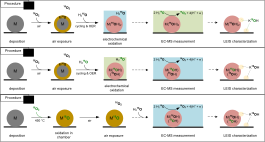
\includegraphics[width=1\textwidth]{04_Oxygen/fig/Strategies_diagram.png}
	\caption{Three strategies for isotope-labeling experiments intended to detect lattice oxygen involvement in the OER, diagrammed for the case of vacuum-synthesized \ch{NiFe} nanoparticles. Taken from Paper \ref{Roy2018}. \textbf{(a)} Strategy A involves mass spectrometric detection of evolved \ch{O2} (EC-MS step) for an unlabeled catalyst in labeled electrolyte. \textbf{(b)} Strategy B involves electrochemical labeling of an OER catalyst followed by EC-MS in an un-labeled electrolyte. \textbf{(b)} Strategy C involves direct preparation (here by annealing in \ch{^{18}O2}) of a labeled electrocatalyst followed by EC-MS in an un-labeled electrolyte.}
	\label{fig:strategies}
\end{figure}


\begin{table}
\begin{adjustbox}{totalheight=\textheight-2\baselineskip}%
	%\resizebox*{!}{\dimexpr\textheight-2\baselineskip\relax}{%
	\begin{tabular}{p{3cm}|p{3cm}|p{2cm}|p{2cm}|p{2cm}|p{2cm}|p{2cm}}
		
		Electrocatalyst & Preparation & Labeling & Electrolyte & Experiment & Result & Citation \\
		\hline
		Pt & On DEMS membrane, oxidized in 98\% \ch{H2^{18}O} & $\le$ 98\% \ch{^{18}O} & Natural 0.5 M \ch{H2SO4} or 1.0 M KOH & LSV, DEMS & no excess \ch{^{18}O} evolved & Willsau, 1985\cite{Willsau1985}\\
		\hline
		Ru and \ch{RuO2}& Sputtered onto Teflon DEMS membrane& Natural & 0.5 M \ch{H2SO4} in 90\% \ch{H2^{18}O} & CVs, DEMS & some excess \ch{^{16}O} evolved &  Wohlfahrt-Mehrens, 1987\cite{Wohlfahrt-Mehrens1987} \\ 
		\hline
		Hydrous \ch{IrO_x} & Thermal decomposition of \ch{HIrCl6} on Ti & Natural & 1 M \ch{HClO4} in 10\% \ch{H2^{18}O} & CVs, DEMS \& chip EC-MS & $>$ 1 ML excess \ch{^{16}O} evolved & Fierro, 2007\cite{Fierro2007}; rep. in Roy, 2018 \\
		\hline
		nanocrystalline \ch{RuO2} and \ch{Ru_{0.9}Ni_{0.1}O_{2-$\delta$}} & (co-)deposition on Ti mesh and annealing & Natural & 0.1 M \ch{HClO4} in 98\% \ch{H2^{18}O}& CVs, DEMS & Some excess \ch{^{18}O} evolved at high $\eta$ & Macounova, 2009\cite{Macounova2009}\\
		\hline
		Molecular Cobaltate Clusters &Electrodeposition of 0.5 mM \ch{Co^{2+}} in labeled phosphate & $\approx$ 87\% \ch{^{18}O} & Natural phosphate buffer& CP, integral headspace& 7-15\% of \ch{^{18}O} loading evolved& Surendranath, 2010\cite{Surendranath2010}\\
		\hline
		\ch{AuO_x} & Au oxidized at 2.0 V in 98\% \ch{H2^{18}O}& $\le$ 98\% \ch{^{18}O}& Natural 1 M \ch{HClO4}& LSV, OLEMS & $\approx$ 1 ML \ch{^{18}O2} evolved & Diaz-Morales, 2013\cite{Diaz-Morales2013} \\ 
		\hline
		polycrystalline, (110), (100), (101), and (111) \ch{RuO2} & oxidized in 98\% \ch{H2^{18}O} & $\le$ 98\% \ch{^{18}O} & Natural 0.1 M \ch{KOH} or 0.1 M \ch{H2SO4} & CVs, OLEMS & Little to no excess \ch{^{18}O} evolved & Stoerzinger, 2017\cite{Stoerzinger2017}\\
		\hline
		Spinel \ch{Co3O4} & as-received & Natural & 0.5 M KOH in 10\% \ch{H2^{18}O} & CVs, DEMS & 34\% ML excess \ch{^{16}O} evolved & Amin, 2017 \cite{Amin2017} \\
		\hline
		Spinel \ch{Co3O4} & electrochemically cycled in 10\% \ch{H2^{18}O} & $\le10\%$ \ch{^{18}O} & Natural 0.5 M KOH & CVs, DEMS & 12\% ML excess \ch{^{18}O} evolved & Amin, 2017 \cite{Amin2017} \\
		\hline
		\ch{LaCoO3} & solid-state synthesis, oxidized in 98\% \ch{H2^{18}O}  & $\le$ 98\% \ch{^{18}O} & Natural 0.1 M KOH & CVs, OLEMS & little to no excess \ch{^{18}O} evolved & Grimaud, 2017\cite{Grimaud2017}\\
		\hline
		\ch{La_{0.5}Sr_{0.5}CoO_{3-$\delta$}}& solid-state synthesis, oxidized in 98\% \ch{H2^{18}O}  & $\le$ 98\% \ch{^{18}O} & Natural 0.1 M KOH & CVs, OLEMS & Some excess \ch{^{18}O} evolved & Grimaud, 2017\cite{Grimaud2017}\\
		\hline
		\ch{Pr_{0.5}Ba_{0.5}CoO_{3-$\delta$}}& solid-state synthesis, oxidized in 98\% \ch{H2^{18}O}  & $\le$ 98\% \ch{^{18}O} & Natural 0.1 M KOH & CVs, OLEMS & Some excess \ch{^{18}O} evolved & Grimaud, 2017\cite{Grimaud2017}\\
		\hline
		\ch{SrCoO_{3-$\delta$}}	& solid-state synthesis, oxidized in 98\% \ch{H2^{18}O}  & $\le$ 98\% \ch{^{18}O} & Natural 0.1 M KOH & CVs, OLEMS & Some excess \ch{^{18}O} evolved & Grimaud, 2017\cite{Grimaud2017}\\
		\hline
		\ch{Ni_{0.75}Fe_{0.25}O_xH_y} film & electrodeposition & Natural & 0.1 M KOH in 97\% \ch{H2^{18}O} & CVs, chip EC-MS  & $\ll$0.1\% lattice O evolution & Roy, 2018\cite{Roy2018a} (Paper \ref{Roy2018})\\
		\hline
		\ch{Ni_{0.75}Fe_{0.25}O_xH_y}, 7 nm nanoparticles & cluster source, electrochem. oxidation & Natural & 0.1 M KOH in 97\% \ch{H2^{18}O} & CVs, chip EC-MS, ISS  & $\ll$0.1\% lattice O evolution & Roy, 2018\cite{Roy2018a} (Paper \ref{Roy2018})\\ 
		\hline
		\ch{Ni_{0.75}Fe_{0.25}O_xH_y}, 7 nm nanoparticles & cluster source, electrochem. oxidation in 97\% \ch{H2^{18}O} & Estimated 50\% \ch{H2^{18}O} & Natural 0.1 M KOH & CVs, chip EC-MS, ISS & $\ll$0.1\% lattice O evolution & Roy, 2018\cite{Roy2018a} (Paper \ref{Roy2018})\\ 
		\hline
		\ch{Ni_{0.75}Fe_{0.25}O_xH_y}, 7 nm nanoparticles & cluster source, thermal oxidation in \ch{^{18}O2} & Estimated 50\% \ch{H2^{18}O} & Natural 0.1 M KOH & CVs, chip EC-MS, ISS & $\ll$0.1\% lattice O evolution & Roy, 2018\cite{Roy2018a} (Paper \ref{Roy2018})\\ 	
		\hline
		Rutile \ch{IrO2} & Reactive sputter deposition with 99\% \ch{^{18}O2}& $\approx$ 99\% \ch{^{18}O} & Natural 0.1 M \ch{HClO4} & CP, OLEMS & little to no \ch{^{18}O} evolved& Geiger, 2018\cite{Geiger2018}\\
		\hline
		Hydrous \ch{IrO_x} & Potential cycling of sputtered \ch{Ir^{18}O2} film in 97\% \ch{H2^{18}O} & $\approx$ 97\% \ch{^{18}O}& Natural 0.1 M \ch{HClO4} & CP, OLEMS & some \ch{^{18}O} evolved& Geiger, 2018\cite{Geiger2018}\\
		\hline
		\normalsize
	\end{tabular}
%}
\end{adjustbox}
	\caption{Isotope-labeling experiments in the water oxidation electrocatalysis literature}\label{tab:lattice_lit}
\end{table}



Table \ref{tab:lattice_lit} shows a list of such experiments reported in the literature. The studies go all the way back to some of the earliest DEMS studies in the 1980's but have accelerated in the past couple years. The experimental methods (catalyst preparation, isotope labeling technique, electrolyte, and isotope exchange experiment measurement technique) are included to aid comparison of the various studies. One clear characteristic of this compilation is that there is no convergence yet in the literature on the best way to conduct these lattice exchange experiments.

The studies are approximately evenly split between DEMS or OLEMS for measuring the evolved oxygen isotopes. Most studies examine the oxygen evolved during potential sweeps (liniear sweep voltammatry, LSV) or cyclic voltammatry (CV), whereas only a few use constant-current measurements (CP). This is a problem because the redox changes during a potential sweep can destabilize electrode materials\cite{Kasian2016, Cherevko2016}, perhaps giving an isotope signal that would not be present in steady-state OER. Of those that measure a lattice oxygen evolution signal, some attempt to quantify the signal in terms of the total or surface oxygen loading of the catalyst\cite{Fierro2007, Surendranath2010, Diaz-Morales2013, Amin2017} whereas many observe an isotope signal but do not quantify it\cite{Wohlfahrt-Mehrens1987, Grimaud2017, Geiger2018}. 

The experiments differ mostly on how the catalyst and electrolyte are isotope labeled. Broadly, there are three strategies:


\begin{itemize}
	\item A. The catalyst is prepared without any labeled oxygen. The lattice oxygen is thus 0.2\% \ch{^{18}O}. Oxygen evolution is then measured in labeled electrolyte with an increased \ch{^{18}O} concentration\cite{Wohlfahrt-Mehrens1987, Fierro2007, Macounova2009, Amin2017, Roy2018a}.
	
	\item B. The catalyst is originally prepared with the natural isotopic ratio, but then it is used for oxygen evolution in a labeled electrolyte. If the OER mechanism involves an exchange between the lattice oxygen and the electrolyte, this will result in labeling of the electrocatalyst with a \ch{^{18}O} concentration in the active lattice sites up to that of the electrolyte. This electrochemically labeled catalyst is then transferred to un-labeled electrolyte, and the isotopic composition of the evolved oxygen is measured.\cite{Willsau1985, Diaz-Morales2013, Stoerzinger2017a, Amin2017, Grimaud2017, Roy2018a}.
	
	\item C. The final strategy is to prepare the catalyst from the start with labeled oxygen, and then measure the isotopic composition of the the \ch{O2} evolved in labeled oxygen. Techniques to synthesize a labeled catalyst include electrodeposition in labeled electrolyte\cite{Surendranath2010}, heating a metal precursor in a \ch{^{18}O2} atmosphere\cite{Roy2018a}, and reactive sputtering with \ch{^{18}O2} in the sputtering plasma\cite{Geiger2018}.
\end{itemize}

These three strategies are illustrated schematically for the case of mass-selected nanoparticles in Figure \ref{fig:strategies}, taken from Paper \ref{Roy2018}. The coming Subsection motivates and describes the isotope labeling studies in that paper.

\subsection{Determining the TOF in NiFe nanoparticles}

As described in Subsection \ref{subsec:NiFe}, our group prepared a model system of vacuum-synthesized, mass-selected \ch{Ni_{0.75}Fe_{0.25}} nanoparticles in order to determine the turn-over frequency (TOF) of nickel-iron based electrodes for water oxidation in alkaline media. The full story is in Paper \ref{Roy2018}. 

\begin{figure}[h!]
	\centering
	\includegraphics[width=1\textwidth]{04_Oxygen/fig/NiFe_redox_vs_surface.png}
	\caption{Activity and redox feature of \ch{NiFeO_xH_y} nanoparticles in 1.0 M KOH. \textbf{(a)}, Turn-over frequencies using three different assumptions about the number of active sites, as a function of particle size. \textbf{(b)}, Cyclic voltammagrams of all samples used for the TOF measurements, zoomed in on the redox feature. \textbf{(c)}, The number of electrons transfered in this redox feature, normalized to the calculated number of surface atoms, as a function of particle size. Taken from Paper \ref{Roy2018}. (a) is from the main text and (b) and (c) are from the SI.}
	\label{fig:redox_vs_surf}
\end{figure}

The activity of nanoparticles for a given (electro)catalytic reaction is influenced by the nanoparticle size\cite{Mistry2016b}. In general, the mass-normalized activity increases with smaller nanoparticle size, as the surface area to volume ratio of a particle increases with decreasing diameter. However, this is not always the case. If, for example, the reaction is most facile a specific type of surface site (for example, if terraces are more active than edges), then there can be an optimum in nanoparticle size. This appears to be the case, for example, in \ch{CO2} reduction to hydrocarbons on copper nanoparticles\cite{Reske2014} and oxygen reduction on platinum nanoparticles\cite{Hernandez-Fernandez2014}. Alternately, if the bulk of a material is active for a reaction, as has been suggested for NiFe-based OER catalysts\cite{Batchellor2015, Doyle2017}, then the mass-normalized activity would not vary with nanoparticle size.

As mentioned in Subsection \ref{subsec:NiFe}, the cluster source synthesis enables us to know the exact mass and surface loading of each sample. Figure \ref{fig:redox_vs_surf}a shows the turn-over frequency at 1.53 V as a function of nanoparticle size vs RHE calculated with three different assumptions about the number of active sites: TOF$_{\text{bulk}}$ assumes all metal atoms are active, TOF$_{\text{surface}}$ assumes metal atoms on the outer surface of the nanoparticle are active, and TOF$_{\text{redox}}$ assumes one active site per electron transfered during the \ch{Ni^{2+}/Ni^{3+/4+}} redox couple just before the onset of OER. This redox couple is shown for all of the samples in the CV's in Figure \ref{fig:redox_vs_surf}b.

Since TOF$_{\text{bulk}}$ (which is proportional to the mass-normalized activity) does indeed decrease with increasing nanoparticle size, we conclude that the bulk of these nanoparticles do not participate in the oxygen evolution reaction. On the other hand, the TOF$_{\text{surface}}$ and TOF$_{\text{redox}}$ do not show clear trends with nanoparticle size. This is consistent with each surface atom being an active site, or with each electron transferred during the redox wave representing an active site. For the electrodeposited NiFe LDH (also described in Subsection \ref{subsec:NiFe}), the exact loading was unknown and so only TOF$_{\text{redox}}$ is shown. This is lower than TOF$_{\text{redox}}$ for the nanoparticles, indicating either that the number of electrons transferred in the redox feature is not the best way to measure the number of active sites, or that the activity of the active sites differ for these two differently synthesized materials.

Figure \ref{fig:redox_vs_surf}c shows the number of redox electrons per Ni atom (black, left y-axis) and per surface Ni atom (red, right y-axis). The latter is equal to the ratio between TOF$_{\text{surface}}$ and TOF$_{\text{redox}}$. For the smallest nanoparticles, the entire nanoparticle appears to be redox active, with approximately one redox electron transferred per nickel atom in the sample, whereas for the larger nanoparticles, there are fewer than 1 electron transferred per nickel atom, indicating that the particles have a redox-inactive core. There are three to five electrons transferred per surface Ni atom, indicating that the redox feature penetrates below the outer surface of the nanoparticles. The question is then whether the redox-accessible portion of the nanoparticle is also OER active. This is illustrated in Figure \ref{fig:NP_diagram}.

\begin{figure}[h!]
	\centering
	\includegraphics[width=0.8\textwidth]{04_Oxygen/fig/NP_diagram.png}
	\caption{Two competing models of the nickel redox feature and oxygen evolution in NiFe nanoparticles. \textbf{Left}, The redox-active near-surface region is permeable to \ch{OH-} and \ch{O2}, and contributes to the OER. \textbf{Right}, The redox-active near-surface region is only accessible by proton shuttling and does not contribute to OER. The diagram on the far left of a proposed layered structure for the redox-permeable NiFeOOH region is from Friebel, 2015, which is Reference \cite{Friebel2015}.}
	\label{fig:NP_diagram}
\end{figure}

The question of whether the redox-active near-surface region contributes to OER is related to the question of which species carries the charge in and out of this region during the redox transition. If it is \ch{OH-}, then it is reasonable to believe that \ch{H2O} and \ch{O2} can also escape, and the near-surface region can contribute to the OER, which in alkaline electrolyte can be written

\begin{equation}
\ch{4 OH- -> O2 + 2 H2O + 4 e-}\,.\label{rxn:OER_alkaline}
\end{equation}

Unfortunately, the transport mechanism involved in the nickel redox feature is still not known\cite{Dionigi2016b}. It is often written by the nominal reaction 
\begin{equation}
\ch{Ni(OH)2 -> NiOOH + (H+ + e- )}\,,\label{rxn:Ni_redox}
\end{equation}
but in addition to protons, hydroxide and solvated cations have all been suggested as possible charge carriers\cite{WehrensDijksma2006}.

We therefore sought to answer the question by another means. We reasoned that, if the redox-active subsurface region participated in the oxygen evolution reaction, then the \ch{H2O} and/or \ch{OH-} originally in that region would be oxidized to \ch{O2} which we could differentiate from oxidation of the bulk electrolyte by isotope labeling. We performed the three isotope-labeling procedures described in Figure \ref{fig:strategies} on mass-selected 7nm NiFe nanoparticles:


\begin{figure}[h!]
	\centering
	\includegraphics[height=0.8\textheight]{04_Oxygen/fig/Roy2018_raw_results.png}
	\caption{EC-MS results for isotope experiments on \textbf{(a-c)} NiFe NP’s (a, b, and c correspond to procedures A, B, and C in Figure \ref{fig:strategies}); and \textbf{(d)} an electrodeposited NiFe thin film and \textbf{(e)} an \ch{IrOx} thin film produced by thermal decomposition of \ch{HIrCl6} in air, by procedure A. The signal for \ch{O2} produced in the largest portion by oxidation of the electrolyte (m/z=36 for procedure A and m/z=32 for procedures B and C) is plotted on the right y-axis, and the other \ch{O2} isotope(s) on the left y-axis. m/z=32 is omitted as a minority isotope since it is dominated by the background due to residual natural \ch{O2}. (f) The excess minority isotope (\ch{^{16}O} for procedure A and \ch{^{18}O} for procedures B and C) is quantified and normalized to (solid bars, left y-axis) the number of surface atoms in the catalyst or to (hashed bars, right y-axis) the total \ch{O2} evolved during the part of the experiment shown here. From the SI of Paper \ref{Roy2018}}
	\label{fig:Roy2018_raw_results}
\end{figure}

For procedure A, the as-synthesized nanoparticles were cycled between 0.5 V and 1.6 V vs RHE in un-labeled electrolyte, to form the hydrated redox-accessible near-surface region implied by Figure \ref{fig:redox_vs_surf}c. The sample was then transferred to the EC-MS setup, where the cell was filled with labeled electrolyte (0.1 M KOH in 97\% \ch{H2^{18}O}), and the potential was cycled up to where oxygen was evolved (1.55 V vs RHE). The advantage to procedure A is that there is no doubt about the initial isotopic composition of the oxygen in the catalyst, as the electrode has only been exposed to natural oxygen. The disadvantage is that the \ch{^{16}O} impurity in the labeled electrolyte limits the sensitivity. 

For procedure B, the as-synthesized nanoparticles were cycled between 0.5 and 1.6 V vs RHE in labeled electrolyte. A disadvantage here is that there is inevitably less than perfect control over the isotopic composition of the electrocatalyst, since it must pass through natural air. We expect, as a worst case, that the oxygen in the catalyst consists of 50\% \ch{^{18}O}, due to formation of \ch{M^{16}O}, with M=\ch{Ni_{0.75}Fe_{0.25}}, when exposed to air and subsequent formation of \ch{M(^{16}OH)(^{18}OH)} when cycled in labeled electrolyte. This is indicated in Figure \ref{fig:strategies}.

For procedure C, the as-synthesized nanoparticles were left in the vacuum chamber, where \ch{^{18}O2} was dosed and the sample was heated to 450$^\circ$C. The nanoparticles were thus already oxidized when taken out into air, and presumably retained a high degree of labeled isotopic purity and the nominal \ch{M^{18}O} formula. However, the sample was then put directly into the EC-MS setup with un-labeled electrolyte, where the nanoparticles likely hydrated to \ch{M(^{16}OH)(^{18}OH)} as illustrated. In hindsight, it would have been better to cycle the particles in labeled electrolyte prior to EC-MS testing to achieve a nominal \ch{M(^{18}OH)2} formula.

In addition to the NiFe nanoparticles, we also tested an electrodeposited NiFe oxyhydroxide film (described in subsection \ref{subsec:NiFe}) in the same electorlyte, and an \ch{IrOx} material produced by thermal decomposition of \ch{HIrCl6}. The latter material was produced by dropcasting a solution of 5 mM \ch{HIrCl6} on a titanium stub and annealing in air at 500$^\circ$C for two hours. This is the same material tested for lattice exchange in Fierro et al, 2007, which is Reference \ref{Fierro2007}. In that study, the authors saw a significant amount of lattice oxygen evolution as an excess \ch{^{16}O} signal during the first cyclic voltammagrams in \ch{^{18}O}-labeled electrolyte (see Table \ref{tab:lattice_lit}). Both the NiFe oxyhydroxide electrodeposited film and the thermal decomposition \ch{IrOx} samples were tested according to Procedure a: They were prepared with the natural isotope ratio, and tested for lattice exchange in labeled electrolyte. The NiFe film was tested in 0.1 M KOH in 97\% \ch{H2^{18}O} like the NiFe nanoparticles. The \ch{IrOx} was tested in 1.0 M \ch{HClO4} in 97\% \ch{H2^{18}O}. The higher concentration of \ch{HClO4} meant that the final isotopic purity of the electrolyte was lower.

The raw EC-MS results for these five isotope-labeling experiments (NP's procedure A-C, NiFe film and \ch{IrOx} procedure A) are shown in Figure \ref{fig:Roy2018_raw_results}a-e. 

Here, a quick note on this plotting form: in this type of isotope labeling experiments, a ''positive'' result is an isotope signal originating from the electrocatalyst, namely a (transient) isotopic composition of the evolved \ch{O2} that cannot be explained by the composition of the electrolyte. A ''negative'' result, on the other hand, is one in which the isotopic composition of the evolved \ch{O2} always reflects the isotopic composition of the electrolyte. It therefore makes sense to plot the results in a way where deviations of the measured \ch{O2} signal and the expected \ch{O2} from oxidation of the electrolyte are clearly visible. After trying a few different plotting strategies, our group thinks that the best way to do so, without hiding any information, is to co-plot the MS signals, scaled according to the expected ratio. This can be done by multiplying one of the signals by the expected ratio, or by using two y-axes scaled according to the expected ratio. The latter technique is used in Figure \ref{fig:Roy2018_raw_results}a-e. In each case, the ''expected ratio'' was taken to be the background-corrected steady-state ratio during a constant-current OER measurement taken right after these cycles.

When plotted this way, it is immediately clear that there is a very small amount of excess \ch{^{18}O} evolved in procedure B (Figure \ref{fig:Roy2018_raw_results}b) in the form of \ch{^{18}O2} (m/z=36) and \ch{^{18}O^{16}O} (m/z=34), a much larger amount of excess \ch{^{16}O} evolved from \ch{IrOx} (\ref{fig:Roy2018_raw_results}e) in the form of \ch{^{18}O^{16}O}, and little to no isotope signal in any of the other samples.

The astute reader may have noticed a rather important experimental mistake: each experiment starts with an anodic scan from OCP, but for the NiFe nanoparticles in both procedures A (Figure \ref{fig:Roy2018_raw_results}a) and C (Figure \ref{fig:Roy2018_raw_results}c), the first cycle does is not anodic enough to produce a significant \ch{O2} signal, and the sample is cycled through the Ni redox couple before a significant amount of \ch{O2} is evolved. If oxygenated species are transferred or mobile during that redox reaction, then the labeled intercallated \ch{OH-} or \ch{O2} might escape to the bulk electrolyte before . We were aware of this mistake while preparing the manuscript, but did not get a chance to repeat these experiments, which were quite challenging for two reasons: (1) The cluster source synthesis was expensive and demanding, and (2) The membrane chips used in the EC-MS experiments at the time were not alkaline-resistant, and so chips would often breach during the measurement. So, after much frustration, we decided to use this data. We concluded, however, that it did not influence the interpretation of the results, for the following reasons: (1) We figured that at least some of the \ch{O} species, such as those bound to nickel in \ch{OH} groups, would stay put during the redox reaction, and (2) The results for procedures A and C were broadly consistent with the results for procedure B (Figure \ref{fig:Roy2018_raw_results}b) and for the electrodeposited film (Figure \ref{fig:Roy2018_raw_results}c), where the anodic potential of the first scan was high enough to give a significant oxygen signal. 

In hindsight, this mistake is part of the simpler and more general mistake of using potential scans rather than constant-potential or (even better) constant-current experiments, since, in general, it is best to hold as much constant as possible when studying a transient phenomenon. In this case, it is best to hold the total \ch{O2} production rate constant when studying potentially transient changes in its isotopic composition.

Figure \ref{fig:Roy2018_raw_results}f shows a quantitative comparison of the five isotope-exchange experiments described in the other panels. The excess lattice oxygen (\ch{^{16}O} for procedure A and \ch{^{18}O} for procedures B and C) is calibrated and normalized to either the number of surface sites (i.e., monolayers, solid bars, left y-axis) or to the total amount of \ch{O2} evolved (right y-axis). In the case of the \ch{IrOx} catalyst, a significant portion ($\approx$ 6\%) of the \ch{O2} contained ''unexpected'' \ch{^{16}O}, indicating that it came from the lattice. For all of the NiFe samples, the portion of the evolved \ch{O2} containing \ch{O} from the lattice was under 0.5\%, with the apparent highest amount coming from the film and the nanoparticles tested by procedure A. Procedure A has the highest expected amount of \ch{^{18}O^{16}} because the purity of the labeled electrolyte ($\le$ 97\% \ch{H2^{18}O}) is less than than the purity of the un-labeled electrolyte ($\approx$ 99.8\% \ch{H2^{16}O}). This indicates that the the apparent portion of evolved \ch{O2} containing lattice O when analyzed by this method is related to the noise level of the m/z=34 signal, i.e., that it doesn't necessarily represent real lattice \ch{O} evolution, which could be zero. The amount of lattice \ch{O} evolved, when normalized to the number of surface sites is $\approx$ 2 monolayers for the \ch{IrOx} catalyst and $\le$ 2\% of a monolayer for all NiFe samples. We concluded therefore, that only the outer surface of the nanoparticles are active, implying that the turn-over frequency closest to the truth is TOF$_{\text{surface}}$, which for the 5.4 nm nanoparticles is $\approx$ 6 s$^{-1}$. This is a record for OER in alkaline electrolyte, as shown in Figure \ref{fig:TOF_alkaline} at the start of this Chapter.

\begin{figure}[h!]
	\centering
	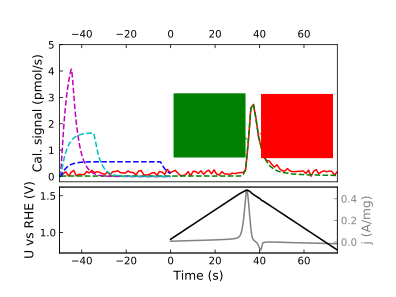
\includegraphics[height=0.8\textheight]{04_Oxygen/fig/NiFe_ECMS_resuls_model.png}
	\caption{\textbf{(a-c)} Analysis of EC-MS results and \textbf{(d-f)} ISS spectra of the samples as-prepared and post-OER for procedures A (a and d), B (b and e), and C(c and f). The experimental procedures are illustrated in Figure \ref{fig:strategies} and the raw EC-MS data is shown in Figure \ref{fig:Roy2018_raw_results}. The modeled signal for 1\% exchange of lattice oxygen should be compared to the \textit{difference} between the expected and measured \ch{^{16}O^{18}O} signal. (a) and (b) are from the main text and (c-f) are from the SI of Paper \ref{Roy2018}}
	\label{fig:Roy2018_model}
\end{figure}

Even if the experimental mistake mentioned above weakens the conclusion that the redox-active near-surface region does not participate in the OER, it does not invalidate these experiments as evidence for the other conclusion of the isotope-labeling experiments: Lattice oxygen is not exchanged during the oxygen-evolution reaction. This is based on an assumption that lattice oxygen is not exchanged during the (near-)surface redox reaction. This may even be used as a definition for lattice oxygen.

To illustrate the sensitivity of the experiments for lattice oxygen evolution, if it occurred, we plotted the data in another way. The majority isotope from electrolyte oxidation (\ch{^{18}O2} for procedure A, \ch{^{16}O2} for procedures B and C) is scaled down according to the isotopic composition of the electrolyte and plotted on the same axes as the other two \ch{O2} isotopic signals, as the ''expected'' m/z=34 signal. The first scan with significant oxygen evolution is shown for each sample.  On the same axes, we plot the expected signal if just 1\% of the lattice \ch{O} were to come out as \ch{O2}. The area of this signal (in pmol) is based on the known metal loading and the nominal formula in Figure \ref{fig:strategies}. The shape is based on the mass transport model in Paper \ref{Trimarco2018}. This modeled signal should be compared to the \textit{difference} in the measured and expected \ch{^{16}O^{18}O} signal. In all cases, it is clear from the difference of the measured and expected signals, and the noise levels, that much less than 1\% of the lattice \ch{O}, if any, is evolved during the first cycle.

Finally, if lattice oxygen is not exchanged during OER, that should mean that it is still present in the catalyst afterwards. To test this we did ion scattering spectroscopy (ISS, also known as low-energy ion scattering, LEIS) on the as-deposited nanoparticle samples, and again after the EC-MS experiment. The results are shown in Figure \ref{fig:Roy2018_model}d-f. The interpretation of the ISS spectra is, in all cases, the interpretation of the ISS spectra is complicated by the fact that some residual potassium, presumably in the form of KOH, is present on the surface of the sample, even after thorough rinsing with ultrapure water (procedures B and C) or labeled water (procedure A). The oxygen in this KOH thus has the isotopic composition of the electrolyte, which is the opposite of that expected in the catalyst. This likely explains the \ch{^{18}O} signal in the ISS spectrum for procedure A (Figure \ref{fig:Roy2018_model}d), whereas we explain the \ch{^{16}O} signal as lattice oxygen which has not exchanged during OER. This is supported by the fact that the \ch{^{16}O}/\ch{^{18}O} ratio increases after the sample is subject to argon sputtering in the vacuum chamber. On the other hand, the potassium signal is much lower in procedues B and C, especially after sputtering, perhaps due to the greater ease of rinsing with non-labeled water. Here, the isotope ratio converges to 1:1, which matches the nominal stoichiometry motivated in Figure \ref{fig:strategies} and the text earlier in this subsection. Together these EC-MS and ISS results make us confident that there is no exchange of lattice oxygen during OER in nickel-iron based catalysts for alkaline water oxidation.

%\clearpage 
\subsection{A contradiction}

The attentive reader may have noticed a contradiction:

In Section \ref{sec:low_O2}, I noted that the acid-electrolyte OER activities of all \ch{RuO2} films and \ch{Ru} foams converged when normalized to the capacitance of the films, which I pointed out is consistent with an assumption that all of the surface area accessible to the electrolyte for active charging is also active for the oxygen evolution reaction. 

However, in Paper \ref{Roy2018}, we argue that only the outer surface of the nanoparticles is active for alkaline-electrolyte OER, even though the Ni redox feature penetrates $\approx$ 3-5 monolayers into the nanoparticles. This argument is quite central to the paper, as the conclusion that catalytic activity is confined to the outer surface of the nanoparticles is used to calculate the record TOF of 6 s$^{-1}$ at an overpotential of 300 mV. In defense of Paper \ref{Roy2018}, we do leave this conclusion somewhat open, and we state clearly the assumptions that is based on. 

We motivate the argument that OER occurs only on the outer surface, and not in the redox-active near-surface region, by isotope-labeling studies that always show \ch{O2} with the same isotopic composition as that of the electrolyte. Our reasoning is that OER activity below the surface would either involve lattice oxygen evolution or oxidation of low-mobility intercalated water. We hypothesize that the redox activity below the surface is only due to proton shuttling.

This contradiction is especially troubling in consideration of the fact that unlabeled \ch{RuO2} films also do not give an isotope signal during OER in isotope-labeled electrolyte. I.e., sputtered \ch{RuO2} also gives a negative result to Strategy A in Figure \ref{fig:strategies}). This is evident, for example, in Figure \ref{fig:He_vs_O2} in the previous Section, where there is no excess \ch{^{16}O} evolution during the first cycles in \ch{^{18}O}-labeled electrolyte (i.e., the m/z=34 to m/z=36 ratio is constant throughout the experiment). Apparently, the water in the porous structure of high-surface-area \ch{Ru} and \ch{RuO2} has no trouble diffusing out of the pores before the onset of OER, unlike our assumption for NiFe oxyhydroxide.

One motivation for these differing lines of reasoning for the two materials is that the porosity is on a different scale: whereas the nanoscale domains and cavities in hydrous \ch{RuO2} are on the order of a few nanometers\cite{Yoshida2013}, the spacing between the layers in \ch{NiFe} layered double hydride are only 0.4 to 0.8 nanometers apart and perhaps interconnected by hydrogen bonds, depending on the phase\cite{Dionigi2016b}. Thus, there is more room for water and other species to diffuse in and out of amorphous \ch{RuO2}. Another is the TEM images of the NiFe nanoparticles (Paper \ref{Roy2018}, Figure 4) which indicate that they are non-porous both before and after the reaction (unfortunately, we do not have TEM images on the sputtered \ch{RuO2} films).

Nonetheless, the uncertainty evident in this contradiction, together with the imperfections mentioned above of the isotope experiments in Paper \ref{Roy2018}, mean that the conclusion of no OER activity in the redox-active near-surface region should be taken with a grain of salt. We think that these issues should motivate research into the charge transfer and mass transport processes during (near-) surface redox reactions at the oxide-electrolyte interface for oxygen evolution catalysts. A better understanding of these transport processes is essential for determining the number of sites that participate in the oxygen evolution reaction, which in turn is essential for developing catalysts with improved intrinsic activity\cite{Kibsgaard2019}. 

\subsection{Labeled \ch{RuO2} films}

As mentioned at the beginning of this Chapter, oxides of iridium and ruthenium and materials based on such oxides are the only known active and somewhat stable oxygen evolution catalysts in acidic electrolyte\cite{Reier2017, Kibsgaard2019}. The electrocatalytic mechanism of such materials has therefore been the subject of many studies, including several using isotope-labeling\cite{WohlfahrtMeherens1987, Fierro2007, Macounova2009, Stoerzinger2017, Grimaud2017}. Some details of these studies are compiled in Table \ref{tab:lattice_lit}.

In Section \ref{sec:low_O2}, I described activity measurements on well-characterized \ch{RuO2} films in isotope-labeled electrolyte (0.1 M 97\% \ch{H2^{18}O}) (effectively giving us procedure A of Figure \ref{fig:strategies} for free), but did not discuss the possibility of lattice oxygen evolution. In contrast, in Figure \ref{fig:Roy2018_raw_results}, I showed a lattice exchange study on a poorly-characterized \ch{IrOx} film formed by thermal decomposition of \ch{HIrCl6}, reproducing the result, first reported in reference \citen{Fierro2007}, of significant lattice oxygen evolution on that material. In this Subsection, I describe isotope-labeling experiments on the \ch{RuO2} materials described in Section \ref{sec:low_O2} as well as sputtered \ch{IrO2} thin films. Sputtered thin films (and cluster source nanoparticles) can be thought of as a model system, in contrast to the more practical but harder-to-understand real catalysts like the thermal-decomposition \ch{IrOx} (and electrodeposited NiFe). Compared to the previous literature, the work presented here adds the high sensitivity of the chip-based EC-MS system as well as surface isotopic characterization by ion scattering spectrometry (ISS).

Part of our motivation for studying OER in acid, in addition to the technological importance of PEM electrolyzers, was a practical consideration: The silicon membrane chips of the EC-MS setup are unstable in alkaline, but stable in acid. Thus, after a frustrating experience involving many experiments being compromised due to chips breaching in the work leading to Paper \ref{Roy2018}, we wanted to work on something (relatively) easy.

\begin{figure}[h!]
	\centering
	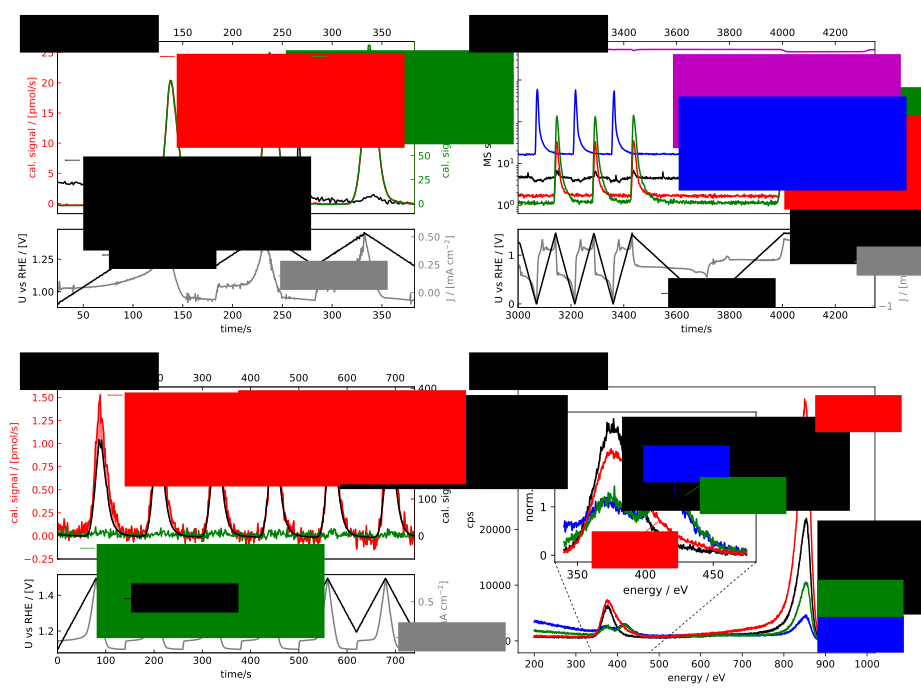
\includegraphics[width=1\textwidth]{04_Oxygen/fig/Reshma1B_lattice_O.png}
	\caption{Lattice oxygen evolution experiments on \ch{RuO2} film sputtered at room temperature with natural \ch{O2}. \textbf{(a)}, The first cyclic voltammagrams of a fresh, un-labeled sample (\ch{Ru^{16}O2}) in labeled electrolyte (0.1 M \ch{HClO4} in 97\% \ch{H2^{18}O}). The left (\ch{^{16}O^{18}O} and \ch{^{16}O2}) and right (\ch{^{18}O2}) y-axes are scaled according to the \ch{^{16}O^{18}O} to \ch{H2^{18}O} measured during steady-state OER later in the experiment. \textbf{(b)}, Electrochemical labeling procedure to incorporate \ch{^{18}O} from the labeled electrolyte into an un-labeled sample. \textbf{(c)}, The first cyclic voltammagrams of in unlabeled electrolyte (0.1 M \ch{HClO4} in 99.8\% \ch{H2^{16}O}) of an electrochemically labeled sample. The left (\ch{^{16}O^{18}O} and \ch{^{18}O2}) and right (\ch{^{16}O2}) y-axes are scaled according to the natural \ch{^{16}O^{18}O} to \ch{H2^{16}O} ratio of 0.40\%. The area between the \ch{^{16}O^{18}O} and (\ch{^{16}O2} signals thus plotted, which is approximately 50 pmol in total on the scale of the left y-axis, is highlighted. \textbf{(d)}, Ion scattering spectra of: (black) a sample that has evolved oxygen in labeled electrolyte (potential holds and cycling between 1.2 and 1.5 V vs RHE) but not brought to reducing potentials; and a sample that has been electrochemically labeled (blue) directly after loading in the vacuum chamber, (green) after 30 minutes of He sputtering, and (red) after 30 minutes of Ar sputtering.
	}
	\label{fig:Reshma1_lattice}
\end{figure}

The isotope-labeling experimental techniques that we used at first on the \ch{RuO2} films were therefore directly taken from those described in the paper above: cyclic voltammatry of un-labeled or electrochemically labeled films, where a  ''positive'' result is a changing isotope ratio during from cycle to cycle. Figure \ref{fig:Reshma1_lattice} shows the results of such experiments on room-temperature sputtered \ch{RuO2} films. The sample was first tested according to Procedure A of Figure \ref{fig:strategies}, i.e., the isotopic ratio was observed during OER from an un-labeled sample in labeled electrolyte. The result, in Figure \ref{fig:Reshma1_lattice}a is that there is no excess \ch{^{16}O} in the evolved \ch{O2} than that expected based on the isotopic composition of the electrolyte. The sample was then tested according to Procedure B, i.e. labeled electrochemically and then tested in un-labeled electrolyte. Procedure B can be more sensitive than Procedure A due to the high isotopic purity (99.8\% \ch{^{16}O}) of natural oxygen. 

Some authors have used steady-state OER as a labeling technique\cite{Stoerzinger2017, Grimaud2017}. This, however, only succeeds in labeling the catalyst if there is a significant amount of lattice exchange, incorporating the oxygen from the electrolyte into the catalyst. And, as shown below, lattice oxygen evolution does not always imply lattice oxygen exchange. Therefore, we used ion scattering spectrometry (ISS) as a direct determination of isotope labeling. The black trace in Figure \ref{fig:Reshma1_lattice}d is an ISS spectrum of an \ch{Ru^{16}O2} film after OER in \ch{^{18}O}-labeled electrolyte (specifically, after the activity test in Figure \ref{fig:Reshma1_activities}b of the previous Section). There is a clear \ch{^{16}O} peak, centered at 375 eV, but no sign of a \ch{^{18}O} peak, indicating that OER does not incorporate oxygen from the electrolyte into the lattice of \ch{RuO2}. This is consistent with the lack of lattice oxygen evolution that has been reported before for crystalline \ch{RuO2}\cite{Stoerzinger2017}, but the (absence of) labeling had not been directly probed. 

Since OER itself did not incorporate the oxygen from the electrolyte into the sample, we instead tried reducing and oxidizing the sample in labeled electrolyte. This procedure is shown in Figure \ref{fig:Reshma1_lattice}b. The sample is cycled between -0.05 V vs RHE, where hydrogen evolution takes place, and +1.4 V vs RHE, where oxygen evolution takes place. This is intended to incorporate the new isotope in the lattice according to the following nominal reactions near the surface of the electrode:
\begin{align}
\ch{Ru^{16}O2 + 4 (H+ + e- ) &-> Ru + 2 H2^{16}O}\nonumber\\
\ch{Ru + 2 H2^{18}O &-> Ru^{18}O2 + 4 (H+ + e- )}\label{rxn:Ru_labeling}
\end{align}
The sample was finally held at 1.4 V vs RHE for 5 minutes to ensure that the surface was oxidized when the sample was removed from electrolyte. 

The blue trace in Figure \ref{fig:Reshma1_lattice}d shows an ISS spectrum of a sample thus labeled. Both oxygen isotopes are clearly present. To ensure that these are not just loosely bound surface species such as adsorbed \ch{H2O} from the electrolyte and/or air, the sample was sputtered in He before taking another spectrum, shown in the green trace. The increase in the \ch{Ru} signal at $\approx$ 850 eV indicates that some surface species are indeed removed, while both oxygen isotopes remain. The presence of \ch{^{18}O} indicates that the surface of the sample was successfully labeled. However, there is still a significant amount of \ch{^{16}O}, indicating that Reactions \ref{rxn:Ru_labeling} are not carried out completely. In other words, the surface is not completely reduced. The approximately 1:1 ratio indicates that 2 electrons are transferred rather than 4 in the (near-)surface redox processes taking place between -0.05 and 1.4 V vs RHE. Using the (110) surface to approximate the surface sites of this polycrystalline sample, the observation of 1:1 \ch{^{18}O}:\ch{^{16}O} in ISS could perhaps indicate exchange of CUS-bound \ch{O} but not bridge-bound \ch{O}. This is consistent with the surface species as a function of potential proposed by Rao et al, 2017, ref. \citen{Rao2017}. In that study, using the ''crystal truncation rods'' of single-crystal x-ray diffraction, the authors show that CUS sites have adsorbed \ch{H2O} at potentials below $\approx$ 0.4 V vs RHE, which would exchange with the electrolyte, whereas bridge sites still have adsorbed \ch{OH}, which would be more tightly bound. Note that this interpretation pushes the definition of ''lattice'' oxygen proposed above, as oxygen that is not exchanged with the electrolyte during surface redox cycling. The definition could be modified to only refer to redox reactions that occur anodic of the electrode's open-circuit potential in air. However, it should also be noted that we are by no means certain of this interpretation - it could be that both CUS and Bridge oxygen atoms are sputtered away by He at the start of the scan, and that ISS only probing oxygen below the adsorbate layer, which would unequivocally be considered lattice oxygen.

To test whether the procedure in Figure \ref{fig:Reshma1_lattice} also labeled the bulk of the sample, we then sputtered the sample with argon for 30 minutes. A separate calibration experiment was done in which a 5 nm \ch{RuO2} film on Ti was sputtered through until the substrate was visible in ISS, taking a total of about 2.5 hours of Ar sputtering with all other parameters held the same. This indicates that 30 minutes of Ar sputtering removes approximately 1 nm of material. The subsequent ISS specrum, the red trace in Figure \ref{fig:Reshma1_lattice} has a much smaller \ch{^{18}O} to \ch{^{16}O} ratio, indicating that there is little to no labeling of the bulk of the material. (We don't believe the Ar sputtering to be completely uniform, so the small amount of remaining \ch{^{18}O} signal probably still comes from the surface and doesn't reflect the isotopic composition exactly 1 nm into the bulk). This sputtering, of course, was destructive to the isotope labeling of the sample, so another sample was labeled by the same procedure for an EC-MS test of lattice oxygen evolution.

Figure \ref{fig:Reshma1_lattice}c shows the oxygen evolved in unlabeled elctrolyte (0.1 M \ch{HClO4} in natural \ch{H2O}) during cyclic voltammatry by a film thus labeled. The axes are scaled according to the natural ratio such that the \ch{^{16}O^{18}O} signal (red trace, left y-axis) and \ch{^{16}O2} signal (black trace, right y-axis) would coincide exactly if all of the oxygen atoms in the evolved \ch{O2} came from the electrolyte. Compared to this baseline, there is clearly some excess \ch{^{16}O^{18}O} in the first cycles, with the isotopic ratio converging to the expected natural ratio after about six cycles. Integrating the excess \ch{^{16}O^{18}O} signal (i.e., the highlighted area in Figure \ref{fig:Reshma1_lattice}c) gives a total of 50 pmol of \ch{O} that must have originated in the lattice. Since the lattice was only 50\% labeled, this would imply that 100 pmol of \ch{O} were evolved. Due to the high surface area of the room-temperature-sputtered films (Figure \ref{fig:Ru_char}), this is only approximately 0.7\% of a monolayer. It is also only $\approx$ 0.1\% of the total \ch{O2} evolved during the first six cycles. 

Our ability to measure lattice oxygen evolution on \ch{RuO2}, in contrast to ref. \cite{Stoerzinger2017}, is due to the labeling procedure and increased sensitivity of the technique, and is not inconsistent with their results. Our ability to quantify the evolved lattice oxygen and compare it both to the number of surface sites and to the total oxygen evolved, enable us to determine that it is negligible with respect to the OER activity. Indeed, the conclusion of the quantitative isotope-labeling studies is that the catalytically relevant OER mechanism on \ch{RuO2} \textit{does not} involve lattice oxygen exchange.



\subsection{Using CO to get out the lattice oxygen}


